
\chapter{Метод исследования}

В работе движение жидкости в круглой трубе воспроизводится численно, путем решения уравнений Навье-Стокса конечно-разностным методом. Возможность адекватного воспроизведения турбулентных течений при решении уравнений Навье-Стокса неоднократно демонстрировалась, начиная с работы \cite{Kim1987}. В частности, в \cite{Priymak1998, Nikitin2006} приведено сравнение полученных численно и экспериментально характеристик развитого турбулентного течения в круглых трубах. В расчетах \cite{Priymak2004} получен турбулентный порыв, его свойства также согласуются с экспериментальными данными. В этой главе приведены математическая постановка задачи, численный метод её решения, некоторые детали реализации метода, а также результаты тестовых расчетов. В тестовых расчетах, выполненных при переходных значениях $\Re$, турбулентность действительно проявляет тенденцию к пространственной локализации; характеристики возникающих локализованных структур согласуются с характеристиками турбулентных порывов, приведенными в литературе. 


\section{Математическая постановка задачи} \label{math_section}

В работе изучается движение жидкости в прямой трубе круглого сечения (жидкость заполняет весь объем трубы). Движение вызывает внешний градиент давления, направленный вдоль трубы. Жидкость считается вязкой и несжимаемой, её плотность $\rho$ и вязкость $\mu$ во всем потоке постоянны. Задача состоит в нахождении скорости жидкости $\v$ и давления $P$ в каждой точке пространства $\x$, заполненного жидкостью, и во времени $t$.

Поле скорости $\v(\x, t)$ удовлетворяет условию несжимаемости:
\begin{equation} \label{eq0}
\div \v = 0.
\end{equation}

Движение жидкости описывают уравнения Навье-Стокса, имеющие с учетом \eqref{eq0} следующий вид:
\begin{equation} \label{NSeq_dynamic}
\pd{\v}{t} = - (\v, \nabla) \v - \frac{1}{\rho}\grad P + \frac{\mu}{\rho} \Laplace \v.
\end{equation}
Уравнения решаются в цилиндрической системе координат $(x,r,\theta)$, где $x$ --- продольное, $r$ --- радиальное и $\theta$ --- угловое направления. 

На твердой стенке трубы радиуса $R$ ставится условие прилипания:
\begin{equation} \label{bc0}
\v = 0 \text{, при } r = R.
\end{equation}

В направлении движения устанавливается условие периодичности с периодом $L_x$. Давление $P$, непосредственно, периодическим не является. Оно представляется в виде суммы периодической $p$ и линейной вдоль трубы $bx$ составляющих. Подстановка $P = p + bx$ в \eqref{NSeq_dynamic} дает уравнение
\begin{equation} \label{NSeq_periodic}
\pd{\v}{t} = - (\v, \nabla) \v - \frac{b}{\rho}\i - \frac{1}{\rho}\grad p + \frac{\mu}{\rho} \Laplace \v.
\end{equation}
Здесь $\i$ -- единичный орт, направленный вдоль трубы. В уравнении \eqref{NSeq_periodic} уже все переменные удовлетворяют условию периодичности вдоль трубы:
\begin{equation} \label{bc1}
[\v, p](x,r,\theta,t) = [\v, p](x+L_x,r,\theta,t).
\end{equation}

Величина $b$ представляет собой внешний градиент давления, который определяется из условия постоянства расхода жидкости $Q$:
\begin{equation}\label{Q_eq}
\int_{S} v_x \, ds = Q.
\end{equation}
Здесь $S$ --- поперечное сечение трубы. Уравнение  \eqref{Q_eq} выполнено в каждом сечении трубы в соответствии с условием несжимаемости \eqref{eq0}. 

Постановка задачи может быть обобщена на случай наличия внешних потенциальных сил $\F = \grad U$. За $b$ в этом случае следует обозначить разность внешнего градиента давления и средней вдоль трубы составляющей внешней силы $F_x$. Не вошедшая в $b$ часть $\F$ потенциальна и имеет вид $\nabla (U - F_x x)$. Разность периодической вдоль трубы части давления и потенциала $(U - F_x x)$ составляет $p$. 

Постановку задачи завершает определение начального поля скорости $\v_0(\x)$, имеющего необходимую гладкость и удовлетворяющего условиям \eqref{eq0}, \eqref{bc0}, \eqref{bc1}, \eqref{Q_eq}. Поставленная задача имеет аналитическое решение, соответствующее ламинарному течению, устанавливающемуся на удалении от входа в трубу. Такое течение называется течением Пуазейля. Оно существует при всех значениях параметров задачи и задается формулой
\begin{equation}
\v = (U (1 - (r / R)^2),\,0,\,0).
\end{equation}
Величина $U = 2U_q$ определяется по расходной скорости $U_q = Q/S$ и соответствует максимальной скорости течения, достигаемой на оси трубы. Градиент давления в этом случае определяется явной формулой
\begin{equation}
b = - 4 \mu U_q R^{-2}.
\end{equation}



В работе все вычисления выполняются в безразмерных переменных. В качестве единиц измерения выступают радиус трубы $R$, максимальная скорость в ламинарном течении $U$ и плотность жидкости $\rho$. Переход к безразмерным переменным, обозначенным штрихами, выполняется по формулам
\begin{equation} \label{dim_less_eqs}
R l' = l, RU^{-1} t' = t, U\v' = \v , \rho U^2 p' = p, \rho U^2 R^{-1} b' = b.
\end{equation}
За $l$ обозначены переменные, имеющие размерность длины, такие как $x, r, L_x$. 

В безразмерных единицах измерения уравнения \eqref{eq0}, \eqref{bc0}, \eqref{NSeq_periodic}, \eqref{bc1}, \eqref{Q_eq} принимают следующий вид (штрихи опущены):
\begin{equation}\label{eq0_Re}
\div \v = 0,
\end{equation}
\begin{equation}\label{NSeq_Re}
\pd{\v}{t} =  - \i b - (\v, \nabla) \v - \grad p + \frac{1}{\Re} \Laplace \v,
\end{equation}
\begin{equation}\label{bc0_Re}
\v = 0 \text{ при } r = 1,
\end{equation}
\begin{equation}\label{bc1_Re}
[\v, p](x,r,\theta,t) = [\v, p](x+L_x,r,\theta,t),
\end{equation}
\begin{equation}\label{Q_Re}
\frac{1}{S} \int_S v_x \, ds = \frac{1}{2}.
\end{equation}
Уравнения \eqref{eq0_Re} -- \eqref{Q_Re} составляют постановку задачи в безразмерном виде. За $\Re = \rho R U / \mu$ обозначено число Рейнольдса, один из двух безразмерных параметров системы. Вторым параметром является $L_x$ --- протяженность расчетной области в продольном направлении. Течение Пуазейля в безразмерных переменных задается более простым выражением:
\begin{equation}
\v = (1 - r^2, 0, 0).
\end{equation}
Безразмерный внешний градиент давления для течения Пуазейля дает формула
\begin{equation}
b = - 4 \Re^{-1}.
\end{equation}

Многие авторы вводят число Рейнольдса иначе, через расходную скорость $U_q$ и диаметр трубы $D$. Несложно показать, что значение числа Рейнольдса, введенного таким образом, совпадает со значением числа Рейнольдса, введенного выше. Однако, например, единица измерения времени $DU_q^{-1}$ в этом случае увеличивается в 4 раза.

В процессе решения задачи возникает необходимость перехода в подвижную систему координат. Выполняя переход, удобно сохранить в качестве тела, относительно которого определяются скорости, стенки трубы. В этом случае граничные условия и значения скорости не зависят от системы отсчета, но в уравнении движения \eqref{NSeq_Re} возникает новое слагаемое, уравнение движения принимает вид:
\begin{equation}\label{NSeq_cf}
\pd{\v}{t} = c_f \pd{\v}{x} - (\v, \nabla) \v - \i b - \grad p + \frac{1}{\Re} \Laplace \v. 
\end{equation}
За $c_f = c_f(t)$ обозначена скорость перемещения системы координат относительно стенок трубы, она может быть функцией времени. Новое слагаемое в \eqref{NSeq_cf} отвечает за перенос решения вдоль трубы со скоростью $-c_f$. Уравнение неразрывности \eqref{eq0_Re} при переходе, выполненном таким образом, как и граничные и начальные условия, не меняется. 

Приведенная постановка задачи традиционна для прямого расчета турбулентных потоков в прямых каналах. В такой постановке удается воспроизводить характеристики течения, устанавливающегося на большом удалении от входа в трубу, решая уравнения движения в ограниченной расчетной области. Условие периодичности вдоль трубы освобождает от необходимости устанавливать условия на входе и выходе из трубы. В тоже время, увеличивая длину периода $L_x$, можно минимизировать влияние этого условия на поток. Для того, чтобы иметь возможность воспроизвести в расчете локализованные турбулентные структуры, необходимо выбирать протяженность расчетной области $L_x$ достаточно большой, не менее $40$ диаметров трубы. 


\section{Численный метод решения поставленной задачи} \label{num_method}

Поставленная задача решается численно конечно-разностным методом \cite{Nikitin2006}. Метод формулируется относительно уравнений движения \eqref{NSeq_Re}, преобразованного к виду:
\begin{equation}\label{NSeq_om}
\pd{\v}{t} =  \v \times \om  - \i b - \grad \Pi - \frac{1}{\Re} \rot \om.
\end{equation}
Здесь $\om = \rot \v$ --- вектор завихренности, посчитанный по полю скорости $\v$; $\Pi = p + \v^2/2$ --- полное кинематическое давление. Эквивалентность уравнений \eqref{NSeq_Re} и \eqref{NSeq_om} следует из векторных тождеств:
\begin{equation*}
-(\v, \nabla) \v = \v \times \rot \v - \grad \frac{\v^2}{2},
\end{equation*}
\begin{equation*}
\Laplace \v = \grad \div \v - \rot \rot \v.
\end{equation*}

Задача решается в цилиндрической системе координат $(x,r,\theta)$. Расчетная область в пространстве $(x,r,\theta)$ имеет форму параллелепипеда:
\begin{equation}
0 < x < L_x, 0 < r < 1, 0 < \theta < 2\pi.
\end{equation}
При решении уравнений в этих переменных необходимо дополнительно установить условие периодичности в направлении $\theta$ и условие ограниченности решения при $r=0$.

В пространстве $(x,r,\theta)$ в расчетной области вводится прямоугольная расчетная сетка, однородная в направлениях $x$ и $\theta$. В радиальном направлении вводится растяжение сетки, что позволяет уменьшить её шаг вблизи стенки. Во всех расчетах, представленных в работе, параметр растяжения выбран таким образом, что размер ячейки в радиальном направлении около стенки в 4 раза меньше, чем в центре трубы. 

При дискретизации уравнений применен подход, при котором различные неизвестные определяются в различных точках сетки. Так, давление $p$ относится к центру ячеек. Компоненты вектора скорости $v_k$ относятся к центрам граней, нормальных к направлению $k$. Компоненты вектора завихренности $\omega_k$ относятся к центрам ребер, параллельных направлению $k$. При таком подходе говорят, что неизвестные определены на смещенных или разнесенных сетках. Он позволяет естественным образом ввести аппроксимацию уравнений второго порядка точности по пространственным переменным.

Пространственная дискретизация вводится таким образом, что сохраняется ряд важных консервативных свойств исходной системы. В частности, тождественно равна нулю дивергенция вязких слагаемых в \eqref{NSeq_Re}, что гарантирует, что это слагаемое не производит массы. Также тождественно равна нулю завихренность градиента давления, что обеспечивает отсутствие влияния давления на эволюцию завихренности непосредственно. 

При моделировании турбулентных течений важно аккуратно воспроизводить изменение кинетической энергии системы. Описывающее его уравнение возникает в результате скалярного умножения на $\v$ уравнений движения \eqref{NSeq_Re} с последующим суммированием по всей расчетной области. Важным свойством системы является то, что в уравнении Навье-Стокса для несжимаемой жидкости градиент периодической составляющей давления и нелинейные слагаемые не производят кинетической энергии, а лишь перераспределяют уже существующую. В конечно-разностной постановке строго выполняются тождества, выражающие этот факт, справедливые при \eqref{eq0_Re}, \eqref{bc0_Re}, \eqref{bc1_Re}:
$$
\int_V \v \cdot \grad p\ d\tau= \int_V \grad (\v p) d\tau = \int_{\Sigma} p v_n d\sigma = 0, 
$$
$$
\int_V \v \cdot (\v, \nabla) \v\ d\tau = \int_V (\v, \nabla)\frac{\v^2}{2}\ d\tau = \int_V \grad (\v \frac{\v^2}{2}) d\tau = \int_{\Sigma} \frac{\v^2}{2} v_n d\sigma = 0.
$$
Здесь $V$ --- расчетная область, $\Sigma$ --- её граница, $v_n$ --- нормальная составляющая скорости на границе. Также строго выполняется дискретный аналог уравнения изменения полной кинетической энергии $E$, записанного в следующем виде:
\begin{equation} \label{Eeq}
\frac{d E}{d t} = - \frac{1}{2}bV - \frac{1}{\Re} \int_{V} \omega^2 d\tau,
\end{equation}
$$
E = \frac{1}{2}\int_{V} \v^2 d\tau.
$$
Изменение полной энергии происходит за счет внешнего градиента давления $b$ и вязкой диссипации. 

Интегрирование по времени выполняется полу-неявным методом Рунге-Кутты третьего порядка точности \cite{Nikitin2006third}. В силу нелинейности оператора Навье-Стокса реализовать полностью неявный метод продвижения по времени затруднительно. Однако наибольшая жесткость системы на достаточно подробных сетках связана с вязким слагаемым. В силу их линейности они могут быть разрешены неявно в то время, как другие слагаемые в операторе Навье-Стокса разрешаются явно. Такой подход называется полу-неявным и позволяет существенно увеличить допустимый временной шаг в сравнении с явными методами. Реализованный алгоритм допускает автоматический выбор шага интегрирования исходя из условия сохранения локальной точности получаемого решения. Таким образом, шаг интегрирования автоматически адаптируется к изменениям в структуре течения, и не требует явного его задания во время счета. 

Неточность выполнения закона сохранения энергии в конечно-разностной постановке может быть следствием не только несовершенства пространственной дискретизации, но и результатом неточности выполнения интегрирования по времени. Метод Рунге-Кутты третьего порядка обладает важным свойством диссипативности --- неточности выполнения шага по времени могут вести лишь к потере кинетической энергии, но не её производству. 

На каждом шаге по времени возникает необходимость по известному полю скорости $\v$ определить полное давление $\Pi$. Для этого необходимо решить уравнение Пуассона, возникающее при условии несжимаемости \eqref{eq0_Re} в результате применения оператора дивергенции к уравнениям движения \eqref{NSeq_om}. Уравнение для определения давления имеет вид:
\begin{equation}\label{P_eq}
\Laplace \Pi = \div \tilde \v,
\end{equation}
$$
\tilde \v =  \v \times \om - \frac{1}{\Re} \rot \om.
$$
Правая часть уравнения \eqref{P_eq} определяется по полю скорости $\v$. Давление также удовлетворяет условию периодичности в направлениях $x$ и $\theta$. На оси трубы значение давления ограничено. Условие на твердой стенке возникает в результате проектирования уравнения \eqref{NSeq_om} на направление нормали $n$:
$$
\pd{p}{n} = \tilde v_n.
$$


Простая геометрия расчетной области позволяет применять прямые методы решения возникающей в результате дискретизации уравнения \eqref{P_eq} линейной системы. Метод решения задачи для давления основан на применении быстрого преобразования Фурье в направлениях $x$ и $\theta$, в которых решение меняется периодическим образом и сетка имеет постоянный шаг. В радиальном направлении система решается методом прогонки. Общая сложность решения задачи для давления составляет $O(N \log N)$, где $N$ --- количество ячеек в расчетной сетке. Решение задачи для давления составляет основную вычислительную сложность используемого метода. 


\section{Реализация численного метода}

Основной пакет программ, используемый при выполнении диссертационной работы, реализующий описанный в предыдущем разделе численный метод, написан на языке программирования fortran77 Н.В. Никитиным. Пакет программ используется в лаборатории общей аэродинамики института механики МГУ уже более 20 лет и хорошо себя зарекомендовал. Программный код отлажен в процессе решении большого числа задач. В частности, с его помощью получены результаты, приведенные в \cite{Nikitin2006}, где демонстрируется совпадение полученных численно характеристик турбулентных потоков в различных геометриях с экспериментальными данными. Качество численного метода и его программной реализации подтверждают также результаты расчета турбулентного течения в трубе при переходных $\Re$, приведенные в следующем разделе. В соответствии с результатами эксперимента, турбулентность принимает форму локализованных структур, характеристики которых совпадают с характеристиками турбулентного порыва. 

Помимо последовательного варианта программы реализован параллельный, позволяющий выполнять расчеты на кластерных вычислительных системах с распределенной памятью. Для коммуникации между процессами, запущенными на различных узлах вычислительной системы, использован интерфейс передачи сообщений MPI ("Message Passing Interface"). Параллельная программа реализована следующим образом. Труба в продольном направлении делится на равные участки, каждый их который хранится в памяти и обрабатывается собственным вычислительным процессом. Существенные временные затраты при выполнении параллельных вычислений связаны с организацией обмена сообщениями между процессами. При решении задачи для давления необходимо выполнить пересылку данных между процессами, при которой каждый процесс обменивается сообщением с каждым. Таким образом, при выполнении одного шага по времени, каждый процессор совершает $O(M)$ пересылок, где $M$ --- число процессов. Затратами на пересылку граничных условий между процессами можно пренебрегать.

Значительная часть расчетов была выполнена на суперкомпьютерах <<Чебышев>> и <<Ломоносов>> суперкомпьютерного комплекса МГУ. Характерное число вычислительных узлов, используемое при расчетах, составляет 32 -- 64, что позволяет увеличить скорость расчетов ориентировочно в 10 раз. 

Значительная часть кода, необходимого при анализе полученных результатов и управлении численными экспериментами, в том числе реализующая метод поиска решения на сепаратрисе (см. раздел \ref{edge_seq}) и метод поиска условно периодических траекторий (см. раздел. \ref{Newton_seq}), была написана на высокоуровневом языке python автором диссертации. Применение указанных методов сводится к последовательному обращению к программе расчета движения жидкости с правильно подобранными начальными данными. 


\section{Методические расчеты} \label{puff_calc}

\begin{figure}[h]
\center{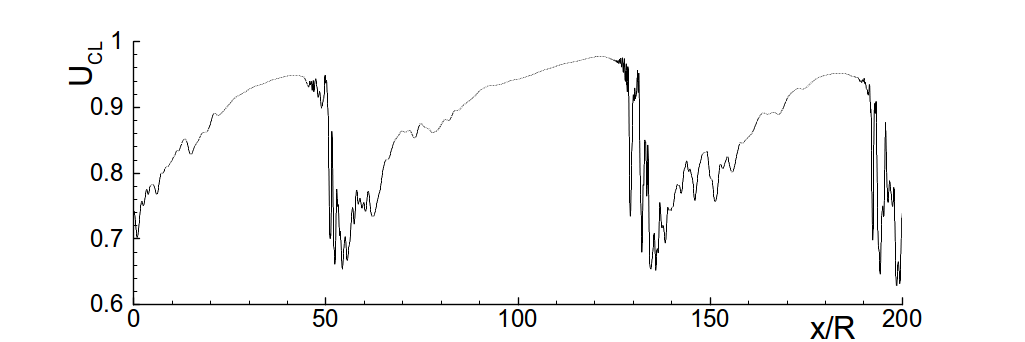
\includegraphics[width=0.9\linewidth]{exper2.png}}
\center{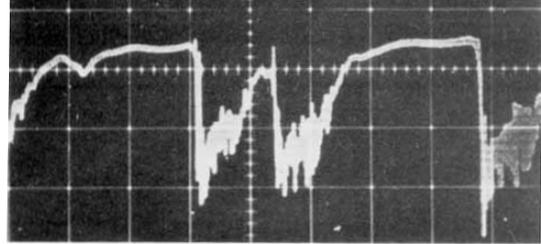
\includegraphics[width=0.68\linewidth]{exper3.png}}
\caption{Сравнение результатов численного расчета и эксперимента. Изображена скорость на оси трубы. Верхний график построен по результатам численного моделирования, выполнено Н.В. Никитиным методом, применяемым в работе. Нижний график получен в эксперименте Вигнанским и Чампайном в 1973 году \cite{Wygnanski1973}.}
\label{exper_img}
\end{figure}

В разделе приведены результаты расчетов движения жидкости в круглой трубе в диапазоне $1670\leqslant Re\leqslant 2800$, полученные при $L_x=200$ с пространственным разрешением $2048 \times 64 \times 128$ в продольном, радиальном и угловом направлении соответственно. Расчеты на более грубой сетке $1024\times32\times64$ во всех рассмотренных случаях дают результаты совпадающие качественно и близкие количественно.

\begin{figure}[h]
\center{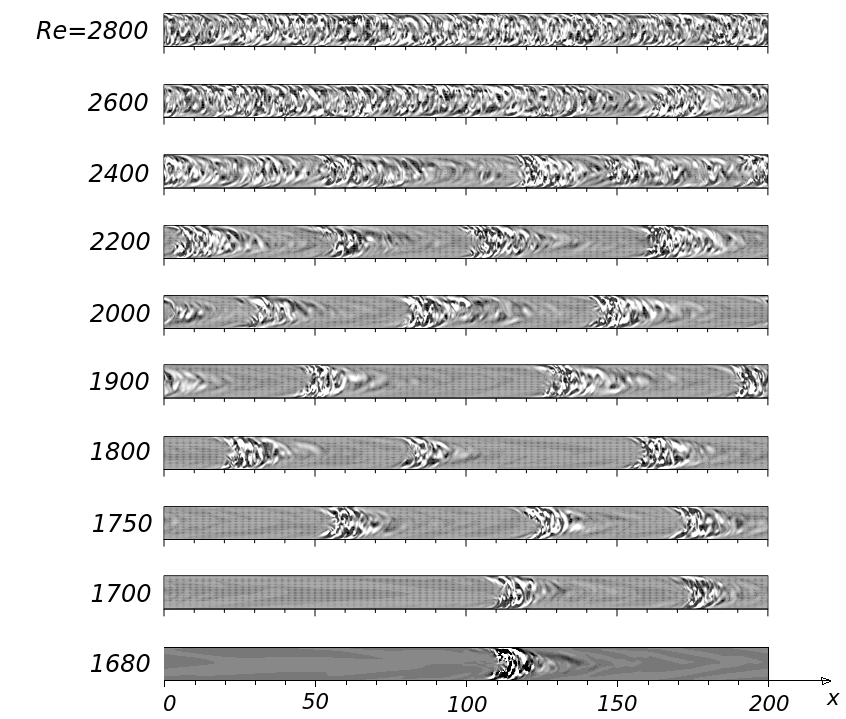
\includegraphics[width=1\linewidth]{puffs.png}}
\caption{Перемежаемый характер турбулентности в трубе в диапазоне переходных чисел Рейнольдса.}
\label{puffs_img}
\end{figure}

Стартуя с начальных данных в виде некоторого трехмерного возмущения течения Пуазейля, уравнения Навье--Стокса интегрируются до выхода решения на тот или иной режим. Установление решения, отвечающего турбулентному течению, происходит в том случае, когда амплитуда начального возмущения достаточно велика, в противном случае возмущения затухают со временем, и решение в конечном итоге возвращается к ламинарному течению Пуазейля. Турбулентный режим за пределами диапазона переходных чисел Рейнольдса $Re\geqslant3000$ имеет вид статистически стационарного процесса и не зависит от конкретного вида начальных условий, при которых он был получен. Течение при этом однородно в продольном направлении, его статистические характеристики согласуются с имеющимися экспериментальными данными (см. рис. \ref{exper_img}). При $\Re\leqslant2600$ в распределении скорости вдоль трубы появляется неоднородность, которая при $\Re\lesssim2200$ приобретает форму двигающейся вдоль трубы цепочки из нескольких пространственно-локализованных структур, разделенных участками ламинарного течения. Конкретное число получающихся в решении турбулентных структур зависит от начальных условий. Кроме того, как было отмечено выше, это число может меняться в процессе эволюции в результате исчезновения или деления отдельных структур. Получаемые в расчетах пространственно-локализованные турбулентные структуры хорошо согласуются с наблюдаемыми в экспериментах турбулентными порывами, что позволяет нам пользоваться этим их наименованием. Отметим, что турбулентные порывы формируются и на некотором отрезке времени существуют в расчетах и при $Re<2000$, вплоть до $Re=1670$. Однако, в этом случае не только число порывов в пределах расчетной области, но и время их существования является случайной величиной и зависит от конкретных начальных условий. Представленная на фиг.~\ref{puffs_img} визуализация рассчитанных течений в диапазоне $1680\leqslant Re\leqslant2800$ демонстрирует эволюцию локализованных структур при изменении числа Рейнольдса.

